\chapter{Assiomi della probabilità}

\section{Spazio campionario ed eventi}
In questa sezione daremo delle definizioni fondamentali per introdurre gli assiomi della probabilità.\\\\
Un \textit{esperimento} è un fenomeno aleatorio come ad esempio il lancio di un dado, l'insieme dei possibili esiti di questo esperimento sono definiti come \textit{spazio campionario}. Un \textit{evento} rappresenta un sottoinsieme dello spazio campionario dato dagli esiti che realizzano l'evento. Dato che gli eventi sono a tutti gli effetti degli insiemi, possiamo applicare tutte le proprietà relative agli insiemi stessi. Siano $E, F$ eventi e $\mathbb{S}$ come spazio campionario con $E, F\subset\mathbb{S}$ allora:
\begin{itemize}
    \item $E\cap F$ è l'evento che si realizza quando sia $E$ che $F$ si realizzano;
    \item $E\cup F$ descrive l'evento che si realizza quando $E$ o $F$ si realizzano;
    \item $E^c=\mathbb{S}\backslash E$ (complemento) è l'evento che si realizza quando $E$ non si realizza.
\end{itemize}

Si definisce \textit{evento certo} un evento che si realizza qualunque sia l'esito ed è rappresentato dallo spazio campionario. L'\textit{evento impossibile}, invece, è l'evento che non si realizza mai qualunque sia l'esito. Due eventi $E$ e $F$ sono \textit{incomparabili} se non possono realizzarsi simultaneamente, ovvero $E\cap F=\emptyset$. Un'evento della forma $\{s\}$ con $s\in\mathbb{S}$ è detto evento \textit{elementare}.

\begin{Example}{}{}
    \textit{Dato l'esperimento del lancio di un dado vediamo come si prestano tutte le precedenti definizioni.}
    
    $\mathbb{S}$: possibili esiti dell'esperimento; \textit{evento}: $E =$ esce un numero pari; $F =$ esce un multiplo di 3. $E\cap F=\{6\}$; $E\cup F=\{2,3,4,6\}$; $E^c=\{1,3,5\}$ esce un numero dispari; \textit{evento certo}: esce un numero da 1 a 6; \textit{evento impossibile}: esce un numero negativo; \textit{eventi incompatibili}: esce un 4 e un 6.
\end{Example}

\section{Assiomi della probabilità}
\begin{redbar}
    Lo \textbf{spazio di probabilità} è una coppia ($\mathbb{S}, P$) dove $\mathbb{S}$ è lo spazio campionario che descrive l'esperimento e $P$, detta funzione di probabilità, è una funzione $E\longmapsto P(E)$ che soddisfa i seguenti \textbf{assiomi}:
    \begin{enumerate}
        \item $0\leq P(E)\leq 1$ $\forall$ evento, ovvero la probabilità di un evento è un numero tra 0 e 1;
        \item $P(\mathbb{S})=1$, la probabilità dell'evento certo è 1;
        \item Data una successione $E_1, E_2, E_3 ...$ di eventi a due a due incompatibili ($\forall i\neq j \mbox{ vale } E_i\cap E_j=\emptyset$) ho:
        \begin{equation*}
            P(\bigcup^\infty_{i=1}E_i)=\sum^\infty_{i=1}P(E_i)
        \end{equation*}
        Questo assioma viene chiamato \textit{additività numerabile}.
    \end{enumerate}
\end{redbar}

Dall'additività numerabile scaturisce l'\textit{additività finita} dove dati $n$ eventi $E_1, E_2, ..., E_n$ a due a due incompatibili (ovvero $\forall i\neq j, E_i\cap E_j=\emptyset$) vale $P(\bigcup^n_{i=1})=\sum^n_{i=1}P(E_i)$.

\begin{Example}{}{}
    \textit{Ho un dado truccato, so che 1 esce con probabilità $0.1$, 2 con $0.3$, 3 con $0.1$, 4 con $0.2$, 5 con $0.2$, 6 con $1.0$. Con che probabilità esce 4, 5 o 6?} 
    
    La riposta è $0.2+0.2+0.1=0.5$ perché $P(\bigcup^3_{i=1}E_i)=\sum^3_{i=1}E_i=0.5$.
\end{Example}

Gli assiomi visti precedentemente generano delle conseguenze che possono essere dimostrate:
\begin{enumerate}
    \item $P(\emptyset)=0$. E' abbastanza banale che la probabilità di un insieme vuoto sia 0 ma vediamo perché:
    \begin{Demonstration}{$P(\emptyset)=0$}{}
        Considero la successione $E_1,E_2,E_3...$ di eventi data a $E_1=\mathbb{S}$ e $E_i=\emptyset$ $\forall i\geq 2$.

        Gli eventi sono a due a due incompatibili (dato che $\emptyset\cap\emptyset=\emptyset$) e per l'assioma di attività numerabile ho $P(\bigcup^\infty_{i=1}E_i)=\sum^\infty_{i=1}P(E_i)$
        \begin{align*}
            \bigcup^\infty_{i=1}E_i=\mathbb{S}\implies P(\bigcup^\infty_{i=1}E_i)=P(\mathbb{S})=1\\
            1=\sum^\infty_{i=1}P(E_i)=P(E_1)+P(E_2)+P(E_3)+...\\
            P(\mathbb{S})+P(\emptyset)+P(\emptyset)+...=1+\infty P(\emptyset)
        \end{align*}
        Ho ottenuto che $1=1+\infty P(\emptyset)$, per l'assioma 1 $P(\emptyset)\in[0,1]$ e l'unico numero che soddisfa questa proprietà è $P(\emptyset)=0$.
    \end{Demonstration}
    
    \item Dimostriamo ora la veridicità dell'additività finita:
    
    \begin{Demonstration}{Additività finita}{}
        Considero la successione $E_1, E_2, ..., E_n, \emptyset, \emptyset, \emptyset$. Quindi $E_i=\emptyset$ per $i\geq n+1$. Gli eventi della successione sono a due a due incompatibili, posso quindi applicare l'additività numerabile $P(\bigcup^\infty_{i=1}E_i)=\sum^\infty_{i=1}P(E_i)$
        \begin{align*}
            \bigcup^n_{i=1}E_i=P(E_1)+P(E_2)+...+P(E_n)+P(\emptyset)+P(\emptyset)
        \end{align*}
        Ho ottenuto che:
        \begin{align*}
            P(\bigcup^n_{i=1}E_i)=P(E_1)+P(E_2)+...+P(E_n)=\sum^n_{i=1}P(E_i)    
        \end{align*}
    \end{Demonstration}
    \item $\forall E$ evento, $P(E^c)=1-P(E)$:
    
    \begin{Demonstration}{$P(E^c)=1-P(E)$}{}
        Osservo che $E$ ed $E^c$ sono eventi incompatibili, cioè $E\cap E^c=\emptyset$. Per l'additività finita ho che $P(E\cup E^c)=P(E)+P(E^c)$. Però $E\cup E^c=\mathbb{S}$ e $P(\mathbb{S})=1$ per il secondo assioma.
        \begin{align*}
            1=P(\mathbb{S})=P(E\cup E^c)=P(E)+P(E^c)\\
            1=P(E)+P(E^c)\hspace{1cm}P(E^c)=1-P(E)
        \end{align*}
    \end{Demonstration}

    \item Dati eventi $E\subset F$, vale $P(E)\leq P(F)$:

    \begin{Demonstration}{$P(E)\leq P(F)$}{}
            Essendo $E\subset F$, $F=E\cup(F\backslash E)$, $E$ e $F\backslash E$ sono eventi incompatibili, cioè $E\cap F\backslash E=\emptyset$. Per l'additività finita $P(E\cup F\backslash E)=P(E)+P(F\backslash E)$ con $P(E\cup F\backslash E)=P(F)$ e $P(F\backslash E)\geq0$ per l'assioma 1. Quindi $P(F)\geq P(E)$.
    \end{Demonstration}
\end{enumerate}

Dati $E$ e $F$ due eventi, $P(E\cup F)=P(E)+P(F)-P(E\cap F)$.
\begin{Demonstration}{}{}
    Notiamo come I, II e III sono a due a due incompatibili e:
    \begin{gather*}
        I=E\backslash F\hspace{1cm}E=I\cup II=P(E)=P(I)+P(II)\\
        II=E\cap F\hspace{1cm}F=II\cup III=P(F)=P(II)+P(III)\\
        III=F\backslash E\hspace{1cm}E\cap F=I\cap II\cap III=P(E\cap F)=P(I)+P(II)+P(III)
    \end{gather*}
    Quindi:
    \begin{gather*}
        P(E\cup F)=P(I)+P(II)+P(III)\\
        P(E)+P(F)-P(E\cap F)=P(I)+P(II)+P(III)-P(II)=\\
        = P(I)+P(III)+P(III)=P(E\cup F)
    \end{gather*}
\end{Demonstration}


In generale se $\mathbb{S}$ è numerabile (infinito o finito) e $P$ è funzione di probabilità allora possiamo calcolare la probabilità $P(E)$ di qualsiasi evento $E$ se conosciamo la probabilità degli eventi elementari. Infatti $P(E)=\sum_{s\in E}P(\{s\})$ e $E=\bigcup_{s\in\{s\}}$ a due a due incompatibili. Per l'additività ho $P(E)=\sum_{s\in E}P(\{s\})$.

\section{Spazi campionari con esiti equiprobabili}
Se ho un esperimento in cui gli esiti hanno la stessa probabilità (equiprobabili) e se $\mathbb{S}$ è finito, allora $\forall E\subset\mathbb{S}$ vale:
\begin{equation*}
    P(E)=\frac{|E|}{|\mathbb{S}|}=\frac{\mbox{\textit{esiti favorevoli}}}{\mbox{\textit{esiti equiprobabili}}}
\end{equation*}

\begin{Proposition}{}{}
    \textit{Se $\mathbb{S}$ è finito e gli esiti sono equiprobabili, allora $\forall E\subset\mathbb{S}$ vale:}
    \begin{equation*}
        P(E)=\frac{|E|}{|\mathbb{S}|}=\frac{\mbox{\textit{esiti favorevoli}}}{\mbox{\textit{esiti equiprobabili}}}
    \end{equation*}
\begin{demonstration}\phantom{}

\begin{itemize}
    \item \textit{Proviamo che $P(\{s\})=\frac{1}{|\mathbb{S}|}$, $\forall s\in\mathbb{S}$}

    Infatti $1=P(\mathbb{S})=\sum_{s\in\mathbb{S}}P(\{s\})$. Chiamiamo $P(\{s\})$ come $c$ e otteniamo $1=\sum_{s\in\mathbb{S}}c=c|\mathbb{S}|$. Quindi $c=\frac{1}{|\mathbb{S}|}$ e siccome $c=P(\{s\})$ ho che $P(\{s\})=c=\frac{1}{|\mathbb{S}|}$.
    \item Sia $E\subset\mathbb{S}$ allora $P(E)=\sum_{s\in E}P(\{s\})$. Ora so che $P(\{s\})=\frac{1}{|\mathbb{S}|}$ e quindi ottengo:
    \begin{equation*}
        P(E)=\sum_{s\in E}P(\{s\})=\sum_{s\in E}\frac{1}{|\mathbb{S}|}=\frac{|E|}{|\mathbb{S}|}
    \end{equation*}
\end{itemize}
\end{demonstration}
\end{Proposition}

\begin{Example}{}{}
    \textit{Lanciando un dado tre volte, qual'è la probabilità $P$ che esce soltanto 2 o 5?}
    
    $\mathbb{S}=\{a_1,a_2,a_3\}$ e $a_{1,2,3}\in\{1,2,3,4,5,6\}$. Per simmetria ha esisti equiprobabili con $E=(a_1,a_2,a_3)$ e $a_i\in\{2,5\}\forall i=1,2,3$. Quindi:
    \begin{equation*}
        P(E)=\frac{|E|}{|\mathbb{S}|}=\frac{2^3}{6^3}=(\frac{1}{3})^3=\frac{1}{27}
    \end{equation*}
\end{Example}

\begin{Example}{}{}
    \textit{Date $n$ persone, qual'è la probabilità $P$ che almeno due hanno lo stesso compleanno?}

    $\mathbb{S}=\{a_1,a_2,...,a_n:a_i\in\{1...365\}\forall i=1...n\}$ e $P(E)=1-P(E^c)$ con $E^c=\{(a_1,a_2,...,a_n)\in\mathbb{S}:a_1,a_2,...,a_n\mbox{ distinti}\}$.
    \begin{equation*}
        P(E)=1-E^c=1-\frac{|E^c|}{|\mathbb{S}|}=1-\frac{365*364*...*(365-n+1))}{365^n}
    \end{equation*}
\end{Example}

\begin{Example}{}{}
    \textit{Estraggo 4 carte da un mazzo di 40, qual'è la probabilità $P$ che siano tutte di bastoni?}

    $\mathbb{S}=\{(a_1,a_2,a_3,a_4):a_i\in\mbox{ mazzo }\forall i=1...4, a_1\neq a_2\neq a_3\neq a_4\}$, per simmetria $\mathbb{S}$ ha esiti equiprobabili ed $E=\{(a_1,a_2,a_3,a_4)\in\mathbb{S}:a_i\mbox{ bastoni}\}$.
    \begin{equation*}
        P(E)=\frac{|E|}{|\mathbb{S}|}=\frac{10*9*8*7}{40*39*38*37}
    \end{equation*}
\end{Example}

\subsection*{Principio di inclusione-esclusione}
Ricordiamo che dati $A$ e $B$ eventi $P(A\cup B)=P(A)+P(B)-P(A\cap B)$. Con tre eventi, invece, $P(A\cup B\cup C)=P(A)+P(B)+P(C)-P(A\cap B)-P(A\cap C)-P(B\cup C)+P(A\cup B\cup C)$.
\begin{figure}[h]
    \centering
    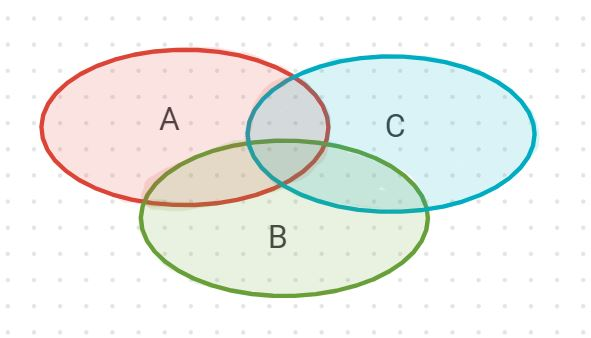
\includegraphics[width=0.5\linewidth]{images/inclusione-esclusione.JPG}
    \label{fig:inclusione-esclusione}
\end{figure}

In generale secondo il principio di \textbf{inclusione-esclusione}, dati $n$ eventi $E_1,E_2,...E_n$ vale:
\begin{align}
    P(E_1\cup E_2\cup...\cup E_n)=&\sum_{i=1}^nP(E_i)-\sum_{1\leq i_1<i_2\leq n}P(E_{i_1}\cap E_{i_2})+\sum_{1\leq i_1<i_2<i_3\leq n}P(E_{i_1}\cap E_{i_2}\cap E_{i_3})...+\notag\\&+(-1)^{n+1}P(E_1\cap E_2\cap...\cap E_n)
\end{align}
    

\section{Probabilità di successioni monotone}
\begin{redbar}
    Una successione di eventi $E_1,E_2,E_3...$ è detta \textbf{monotona} se è crescente o decrescente. In particolare è crescente se $E_1\subset E_2\subset E_3...$, mentre è decrescente se $E_1\supset E_2\supset E_3...$    
\end{redbar}

Data una successione monotona di eventi $E_1,E_2,E_3...$, l'evento limite $\lim_{n\to\infty}E_n$ è definito come:
\begin{equation*}
    \lim_{n\to\infty}E_n:=\bigcup_{n=1}^\infty E_n\hspace{1cm}\lim_{n\to\infty}E_n:=\bigcap_{n=1}^\infty E_n
\end{equation*}
se la successione è rispettivamente crescente o decrescente.

\begin{Thm}{Successioni monotone}{}
    \textit{Data una successione monotona di eventi $E_1,E_2,E_3...$ vale:}
    \begin{equation*}
        P(\lim_{n\to\infty})=\lim_{n\to\infty}P(E_n)
    \end{equation*}
    \begin{equation*}
        \lim_{n\to\infty}E_n:=\begin{cases}\bigcup^\infty_{n=1}E_n\mbox{ se } E_1\subset E_2\subset E_3\subset ...\\\bigcap^\infty_{n=1}E_n\mbox{ se }E_1\supset E_2\supset E_3\supset ...\end{cases}
    \end{equation*}
\begin{demonstration}
    Su $E_1\subset E_2\subset E_3\subset ...$ ho una successione monotona crescente di eventi. 
    \begin{equation*}
        F:=\lim_{n\to\infty}E_n\hspace{0.5cm}\mbox{ quindi }\hspace{0.5cm}F=\bigcup^\infty_{n=1}E_n
    \end{equation*}
    \begin{minipage}{\textwidth}
        \centering
        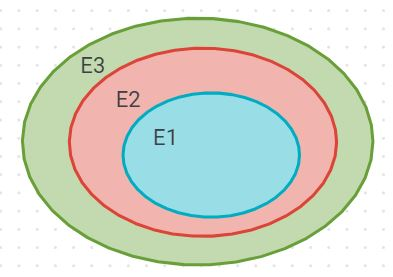
\includegraphics[width=0.5\linewidth]{images/successioni-monotone.JPG}
        %\captionof{figure}{Esempio di esecuzione di un programma}
        \label{fig:successioni-monotone}
    \end{minipage}\\\\
    $A_1=E_1$, $A_2=E_2\backslash E_1$, $A_3=E_3\backslash E_2$, ..., $A_n=E_n\backslash E_{n-1}$ perché $A_1,A_2...$ sono a due a due disgiunti.
    \begin{equation*}
        E_n=A_1\cup A_2\cup...\cup A_n\hspace{1cm}F=\bigcup_{n=1}^\infty E_n=A_1\cup A_2\cup A_3\cup ...
    \end{equation*}
    Quindi ho \circled{1} per additività finita e \circled{2} per additività numerabile:
    \begin{align*}
        \circled{1}P(E_n)=\sum^n_{k=1}P(A_k)\hspace{1cm}\circled{2}P(F)=\sum^\infty_{k=1}P(A_k)\hspace{1cm}\circled{3}\sum^\alpha_{k=1}P(A_k)=\lim_{n\to\infty}\sum^n_{k=1}P(A_k)
    \end{align*}
    Combinando \circled{1}, \circled{2} e \circled{3} ho $P(F)=\lim_{n\to\infty}P(E_n)$, abbiamo così dimostrato il teorema per le successioni crescenti di eventi.\\\\
    Sia ora $E_1\supset E_2\supset E_3\supset ...$ una successione monotona decrescente definisco:
    \begin{equation*}
        G_n:=E_n^c=\mathbb{S}\backslash E_n\hspace{0.5cm}\mbox{ allora }\hspace{0.5cm}G_1\subset G_2\subset G_3\subset...
    \end{equation*}
    Applico il teorema della successione crescente per $G_n$ con $n\geq1$ e ottengo (dato che la successione è decrescente):
    \begin{align*}
        P(\bigcup^\infty_{n=1}G_n)=\lim_{n\to\infty}P(G_n)\hspace{0.5cm}\mbox{ quindi }\hspace{0.5cm}1- P(\bigcup^\infty_{n=1}G_n)=\lim_{n\to\infty}[1-P(G_n)]
    \end{align*}
    applicando De Morgan:
    \begin{equation*}
        P((\bigcup^\infty_{n=1}G_n)^c)=P(\bigcap^\infty_{n=1}G_n^c)=P(\lim_{n\to\infty}E_n)
    \end{equation*}
    Quindi:
    \begin{equation*}
        P(\lim_{n\to\infty}E_n)=\lim_{n\to\infty}P(E_n)
    \end{equation*}
\end{demonstration}
\end{Thm}

\begin{Example}{}{}
    \textit{Immaginiamo un esperimento ideale in cui si lancia infinite volte una moneta. Un esito è una successione dove $x_n\in\{T,C\}$ e $x_n$ è il risultato del lancio n-esimo. Con $\mathbb{S}=\{(x_1,x_2,...):x_i\in\{T,C\}\}=\{T,C\}^{\mathbb{N}_+}$ qual'è la probabilità $P$?}

    La definizione di questo $P$ si basa su un lavoro teorico che va oltre questo coso. Diamo per assodato che esista $P$ funzione di probabilità che descrive bene questo esperimento ideale.

    Fissiamo $(a_1,a_2,a_3,...)\in\{T,C\}^{\mathbb{N}_+}$ e $P(\{(a_1,a_2,a_3,a_4,...)\})$ (ad esempio esce sempre Testa). Con $E_n=\{\mbox{eventi di n lanci fino all'n-esimo}\}$, $P(E_n)=\frac{1}{2^n}$.

    Dato che gli eventi sono sempre più limitanti ($E_1\supset E_2\supset E_3\supset...$), per il teorema di continuità:
    \begin{equation*}
        \{(a_1,a_2,a_3,...)\}=\bigcap^\infty_{n=1}E_n\hspace{1cm}P(\{(a_1,a_2,a_3,...)\})=\lim_{n\to\infty}P(E_n)=\lim_{n\to\infty}\frac{1}{2^n}=0
    \end{equation*}
    Quindi $\forall s\in\mathbb{S}$ ho $P(\{s\})=0$
\end{Example}